\authoredSection{alex}{Vorgehen}
\subsection{Orientierungsphase}
	Zu Beginn des Vorgehens standen Ideenfindung, Konzeption, Lernprozesse und das Finden eines gemeinsamen Arbeitsrhythmusses im Vordergrund. Eine erste grobe Orientierung, welche Aufgabenteile die einzelnen Beteiligten der Gruppe im Verlauf annehmen würden, ergab sich nach der „Kick-Off“-Veranstaltung bei T-Systems. Die Kompetenzen des Teams wurden anschließend auf die Positionen des Entwicklers, Konzepters, Projektleiters und Beraters aufgeteilt. 
	
	Zum Zeitpunkt der Ideenfindung wurde das Vorgehen noch weniger zentral organisiert, als es später durch den Projektleiter realisiert werden sollte. Es galt zunächst herauszufinden, mit welchen konkreten Aufgaben man sich im weiteren Verlauf konfrontieren konnte. Um eine grundlegende Kommunikation zwischen den Teammitgliedern zu etablieren, wurde eine Facebook-Gruppe gegründet, die dazu diente Ideen festzuhalten, zu besprechen und Termine oder Aufgaben für kommende Treffen zu vereinbaren. Um die Ideen darüber hinaus geordnet aufzuschreiben und für alle Beteiligten abrufbar zu machen, wurde zusammen mit dem Coderepository ein Wiki bei Github angelegt, siehe Abbildung \ref{fig:WikiHome}. Das Wiki fand im Speziellen in dieser frühen Phase Verwendung.
	
\begin{figure}[h]
	\centering
	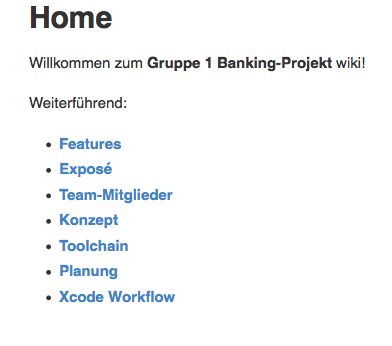
\includegraphics[width=6cm]{Pictures/wiki_home}
	
\includegraphics[width=6cm]{Pictures/wiki-konzept}
	\caption{Wiki bei Github\label{fig:WikiHome}}
\end{figure}

	Neben der Formfindung von Konzepten diente das Wiki ebenfalls auch zum Festhalten von Code-Style Konventionen (NYTimes Objectvice-C-Style Guide) oder Workflows, wie etwa dem toolunterstützten Erstellen von Doxygen-kompatiblen Methodenkommentaren mit dem Xcodeplugin VVDocumenter\footnote{\url{https://github.com/onevcat/VVDocumenter-Xcode}}. Auf Basis des Letzterem ließe sich bei Bedarf aus den Kommentaren eine Dokumentation im html-Format generieren. 

	Einen der ersten Schritte im Arbeitsprozess nach Erstellung des Exposés konnten wir mit Hilfe einer Umfrage bezüglich der Kundenbedürfnisse, -erwartungen und -bedenken respektive des Genres der Applikation, sowie unserer spezifischen Vorstellung, sprich der möglichen Features des Endprodukts, erreichen. Im Rahmen der ersten internen Treffens des Teams und der Plenumsveranstaltungen konnten sich die Vorstellungen langsam konkretisieren. Deutlich wurde dabei, wie diese zu priorisieren sind und welche Einschränken (wie bspw. Sicherheitsaspekte, Wertigkeit des Features) an eine mögliche Umsetzung geknüpft sind. In diesem Prozess wurde das Konzept stetig auf die Rückmeldungen der Plena angepasst. Begleitet wurde das Vorgehen durch das Erstellen von Mockups, die bereits in diesem Stadium helfen konnten, Inhalte nicht zuletzt visuell zu vermitteln und zu besprechen. Die Verwendung von Mockups fand aber auch im weiteren stets Anwendung, um Skizzen für eine mögliche Visualierung zu erstellen, bevor diese final umgesetzt wurden.

	Besonderes Augenmerk lag in der frühen Phase bezogen auf das Konzept im Herausarbeiten eines Alleinstellungsmerkmals durch das sich mit Hilfe der Applikation die Fililalbank von der Direktbank positiv abheben kann. Dieser Punkt markierte gewissermaßen bei unserem Team die Hürde, um mit der eigentlichen Umsetzung zu beginnen. Die Featureideen sortierten wir fortlaufend neu nach geschätzter Priorität. Im Wiki unterschieden wir dabei grundsätzlich zwischen „Major“ und „Minor“.  
	
	Mit den Major-Features sollten die Kernfunktionalitäten der Applikation beschrieben werden. Hierzu zählten unter anderem der Filialfinder, der individuell angepasste Kreditrechner, sowie später primär fokussiert der Self-Service. Features, welche die App in der Gesamtheit aufwerten sollten aber nicht zur Kernfunktionalität gehören, bildeten die Minor-Kategorie. Ein Beispiel hierfür ist die Überweisungsfunktion für Girokonten. Sie wird in diesem Kontext erwartet, stellt aber keine Möglichkeit zur Abgrenzung gegenüber ähnlichen Anwendungen dar. Sie trägt außerdem nicht direkt dazu bei, die übergeordnete Fragestellung den Kunden wieder mehr an die Filialbank zu binden, zu erfüllen. Im Rahmen der Priorisierung verdeutlichte sich des weiteren, welche Features später nicht umgesetzt würden. Ein Feature das aufgrund niedrig eingestufter Priorität nicht den Weg bis in das Endprodukts geschafft hat, ist bspw. der SEPA-Umrechner, der das zuvor bestehende Format in die neue Kodierung umrechnen sollte. 
	
	Ebenfalls gab ausgedehnte Überlegungen, ob die Software für iPad, iPhone oder sogar dual für beide Geräte entwickelt werden sollte. Wie bei den Features war es auch hier hilfreich, wenn auch nicht einfach, demokratisch über eine Entscheidung abzustimmen. Dies zog auch nach sich, dass das Kollektiv den Einzelnen teils entgegen seiner eigenen Überzeugung zu einer gemeinsamen Lösung drängte. 
	
	Da die Kernfrage der Kundenbindung an die Filialbank schwer zu beantworten war, kam die Fragestellung des Zielgeräts und der damit verbundenen Auswahl an Features nach einer zuvor vermeintlich finalen Entscheidung mehrmals auf. Schlussendlich fiel die Entscheidung auf das iPad, weil wir die Kernfeatures durch dieses besser abdeckt sahen und sich nach der Umfrage der Eindruck einstellte, dass Nutzer sicherheitskritische Anwendungen bevorzugt in Ruhe Zuhause statt unterwegs verwenden wollen. Der Entschluss, sich bei der Entwicklung auf ein Gerät zu fokussieren, wurde teamintern unter den Gesichtspunkten mangelnden Gewinns einer dualen Entwicklung und dem damit verbundenen zusätzlichen Aufwand entschieden.

\subsection{Umsetzungsphase}
	Nachdem das grundlegende Konzept ausgearbeitet war, konnten wir mit der konkreten Umsetzung beginnen. Infolgedessen musste sich das Team auf einen Satz von Tools einigen, mit denen die Entwicklungsaufgaben verwaltet, zugeteilt und festgehalten wurden. Initial fiel die Entscheidung auf eine Kombination von Google-Docs und Github-Issues/Milestones. In Github lassen sich sog. Issues definieren. Diese Issues stellen Aufgaben dar, die Mitgliedern des Teams zugewiesen werden. Einzelne Issues werden wiederum Zwischenzielen zugewiesen, den Milestones. Sind alle Issues bezüglich eines Milestones abgearbeitet, ist dieses erfüllt. Die Verwaltung und Verteilung der Aufgaben wurde von diesem Zeitpunkt an durch den Projektleiter zentral durchgeführt. Alle neu entstehenden Aufgaben wurden also immer in Absprache mit diesem in das Issuesystem eingefügt. Dies war für die Übersicht der kommenden Aufgaben, verbunden mit der Gewissheit, dass alle Mitglieder über den Fortschritt im Ganzen wie im Einzelnen den gleichen Informationsstand haben, eine echte Hilfe. Die in Github eingetragenen Issues wurden neben der Zuweisung an Personen mit Labels versehen, die zum einen die Priorität zum anderen, das Überthema der Aufgabe beschreiben. Hochprior wurde u.A. das Erstellen einer Basisarchitektur auf der im weiteren softwaretechnisch aufgebaut werden sollte, sowie das Beschreiben der vorkommenden Entitäten und der damit verbundenen Relationen eingestuft. 

	Während wir GitHub zum Zuteilen und Festhalten der Aufgaben einsetzten, konnte mit Google-Docs der zeitliche Aufwand dafür festgehalten werden. Pro Aufgabe wurde eine Zeile mit entsprechendem Titel angelegt. Falls vorhanden, ist in der Tabelle das korrespondierende GitHub-Issue mit Verlinkung eingetragen. Die den Aufgaben zugewiesenen Teammitglieder sind mit Initialen vermerkt. Aus der tatsächlich aufgewendeten Zeit multipliziert mit der Anzahl der zugeteilten Personen resultiert der kumulierte Aufwand. Die Vorstellung der zu erledigenden Arbeiten war zu diesem Zeitpunkt allerdings meist unvollständig konkretisiert. Davon abgesehen gab es keine Vorerfahrungen bezüglich des iOS-Frameworks. Entsprechend mussten wir davon ausgehen, dass Aufwandsschätzungen zu Beginn nur bedingt hilfreich sein konnten. Trotzdem war dies als Vorlauf evtl. wichtig, um im  weiteren Verlauf ein gutes gemeinsames Verständnis für die Dokumentation und Verwaltung des Arbeitsaufwands zu entwickeln und zu präzisieren. 

\begin{figure}[h]
	\centering
	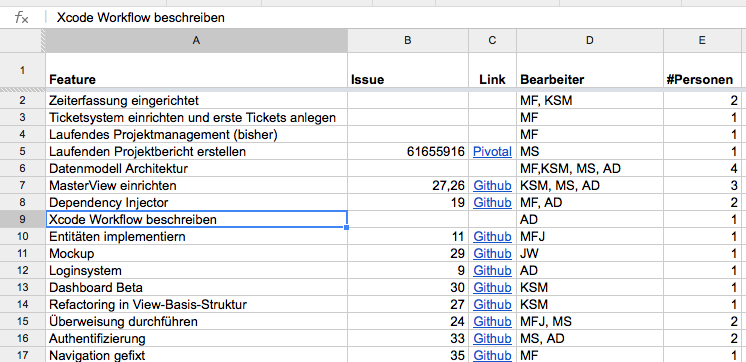
\includegraphics[scale=.25]{Pictures/gdocs1} \\
	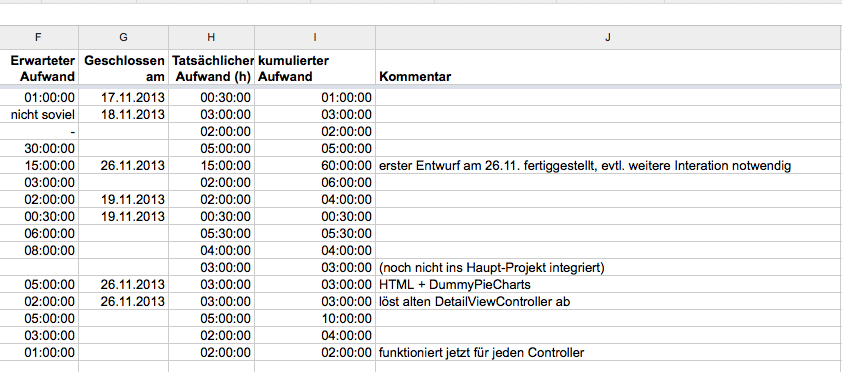
\includegraphics[scale=.25]{Pictures/gdocs2}
	\caption{Google Doc\label{fig:GDoc}}
\end{figure}

	Während der Anfangsphase etablierte sich im Team ein Arbeitsrhythmus mit zwei Terminen pro Woche, in denen jeweilig das Arbeitspensum eines Werktages oder darüber hinaus absolviert wurde.  Die zeitlichen Gegebenheiten mussten auf unsere Gruppe von Studenten mit je unterschiedlichen Stundenplänen abgestimmt werden. In voller Gruppenstärke war es, abgesehen von Ausnahmen, folglich kaum möglich, außerhalb der festen Projekttermine zusammenzukommen. Um in unseren Arbeitsabläufen dennoch Kontinuität herzustellen, haben wir die vereinbarten Termine entsprechend organisiert, dass mindestens die Hälfte der Gruppe anwesend sein konnte. Folglich wurden die Termine alternierend in unterschiedlichen Besetzungen durchgeführt. 

	Die frühen Teamtreffen waren neben den eigentlichen Aufgabenstellungen stark davon geprägt, sich mit Objective-C, dem iOS-Framework sowie der Entwicklungsumgebung vertraut zu machen. Vielleicht wurde auch infolge dessen zunächst primär eine technische Umsetzung unter Vernachlässigung visueller Aspekte versiert. Nach der Rückmeldung in einem der frühen Plenumstermine, dass visuelle Gestaltung der technischen zeitlich nicht nachsteht und parallel dazu entwickelt werden sollte, wurde die Arbeitsweise dahingehend umgestellt. Technische und visuelle Gestaltung wurden von diesem Zeitpunkt an gleichzeitig entwickelt. 

\subsection{Vorgehensweise nach Scrum}
	Im Anschluss an die Scrum-Zertifizierung wurden Arbeitsabläufe und Positionierung der Mitglieder im Team erneut reflektiert, um einen Scrum-Prozess mit den entsprechenden Rollen zu realisieren. Korrespondierend zu den zuvor zugewiesenen Positionen des Entwicklers, Projektleiters, Beraters und Konzepters wurde nach Äquivalenten in der Scrum-Terminologie gesucht. Entwickler und Konzepter wurden der Gruppe des Development Teams zugeteilt. Während beim Berater eine Analogie zum Scrum Master gebildet wurde, lag es nahe, den Projektleiter dem Product Owner zuzuordnen. 

	Bereits vor der Zertifizierung hatte sich durch den Scrum Master die Praxis eines Daily Scrums eingestellt. Das Daily Scrum Meeting wurde immer zu Beginn jedes Treffens umgesetzt. Dies brachte den positiven Effekt mit sich, dass trotz alternierender Besetzungen sich alle Mitglieder zu Arbeitsbeginn über den aktuellsten Stand ausgetauscht hatten. Der Product Owner zuvor Projektleiter verwaltete weiterhin wie zuvor beschrieben zentral das Aufgabenmanagement. 
Problematisch erwies sich die zuvor getroffene Toolauswahl zur Organisation der Aufgaben unter den Gesichtspunkten von Scrum. Primär fehlte es den Tools an Möglichkeiten der Idee des iterativen Sprints gerecht zu werden. Infolgedessen stellte das Team die gesamte Toolchain zur Verteilung der Aufgaben und deren Aufwandsmessung um. Die Wahl fiel auf das Tracking-Tool PivotalTracker, in welchem die Terminologie Scrums mit Sprint-Backlog, Sprint-Velocity, „Done“- Status, usw. vertreten war. Die zuvor erstellten Issues und Aufwandseinschätzungen der noch offenen Aufgaben wurden komplett in die neue Umgebung übertragen.

\begin{figure}[h]
	\centering
	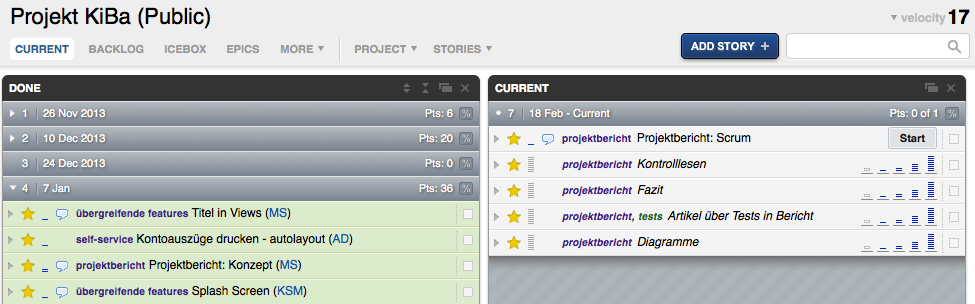
\includegraphics[scale=.25]{Pictures/pivottracker-overview}
	\caption{Stories bei PivotalTracker\label{fig:Pivottracker}}
\end{figure}

	Als Iterationsdauer legten wir einen Zeitrahmen von zwei Wochen fest. Diese Dauer erschien uns als sinnvoll; einerseits lang genug um, kleine oder mittelgroße Aufgaben innerhalb einer Iteration zu bewerkstelligen, anderseits nicht zu lang, um dynamisch auf geänderte Anforderungen reagieren zu können, ohne den Sprint-Backlog innerhalb eines Sprints modifizieren zu müssen. 
	
	Der Prozess des dynamischen Reagierens auf Kritik und sich damit ändernden Anforderungen vollzog sich über die gesamten Zeitspanne des Projekts. Das stetige Überdenken und Anpassen voriger Überlegungen und Ausarbeitungen stellte sich als eine der größten, wenn nicht als die größte Herausforderung des Projekts dar. Eine ständige Korrektur führt auch zum Verwerfen voriger Arbeit, woraus die Anforderung entsteht, sich stetig für neue Richtungswechsel zu motivieren.  

	Nach der Anfangsphase wurden die Aufwandsschätzungen präziser. Weiterhin war es zwar schwierig, genaue Schätzungen für einzelne Aufgaben vorzunehmen, insgesamt konnten wir aber trotz alledem auf Basis der sich ergebenden Sprint-Velocity ab dem letzten Drittel des Semesters eine sinnvolle Einschätzung über den verbleibenden Arbeitsaufwand und die dafür benötigte Zeit abgeben. Wie sich herausstellte, konnten wir diese Einschätzung auch einhalten. 

	Bezüglich der strengen Richtlinien von Scrum – entweder es wird auf voller Linie praktiziert oder aber das Vorgehensmodell ist nicht eingehalten und somit auch anders zu benennen – ist noch erwähnenswert, dass diese eigentlich vorsehen, dass das Development Team zu Beginn seiner Arbeit bereits alle notwendigen technischen Kompetenzen zur Umsetzung eines Projekts besitzt. Wir waren allerdings damit konfrontiert, selbstständig fortlaufend Wissen zu erarbeiten, das zur Bewältigung der Aufgaben notwendig war. Davon abgesehen war das Team auch in weiteren Punkten nicht durchweg sicher, ob es alle Vorgaben des Modells einhalten könne.

	 Neben den erwähnten Vorteilen des Tracking-Tools, respektive Struktur und Terminologie, ermöglichte uns die neue Umgebung das Verhältnis von bestehenden und noch zu erledigenden Aufgaben in Balkendiagrammen und Burndown-Charts zu visualisieren. Der Burndown-Chart bzw. Progress-Report über die gesamte zweite Hälfte der Projektdauer ergibt sich wie folgt:
	 
\begin{figure}[h]
	\centering
	\hspace{1.6cm}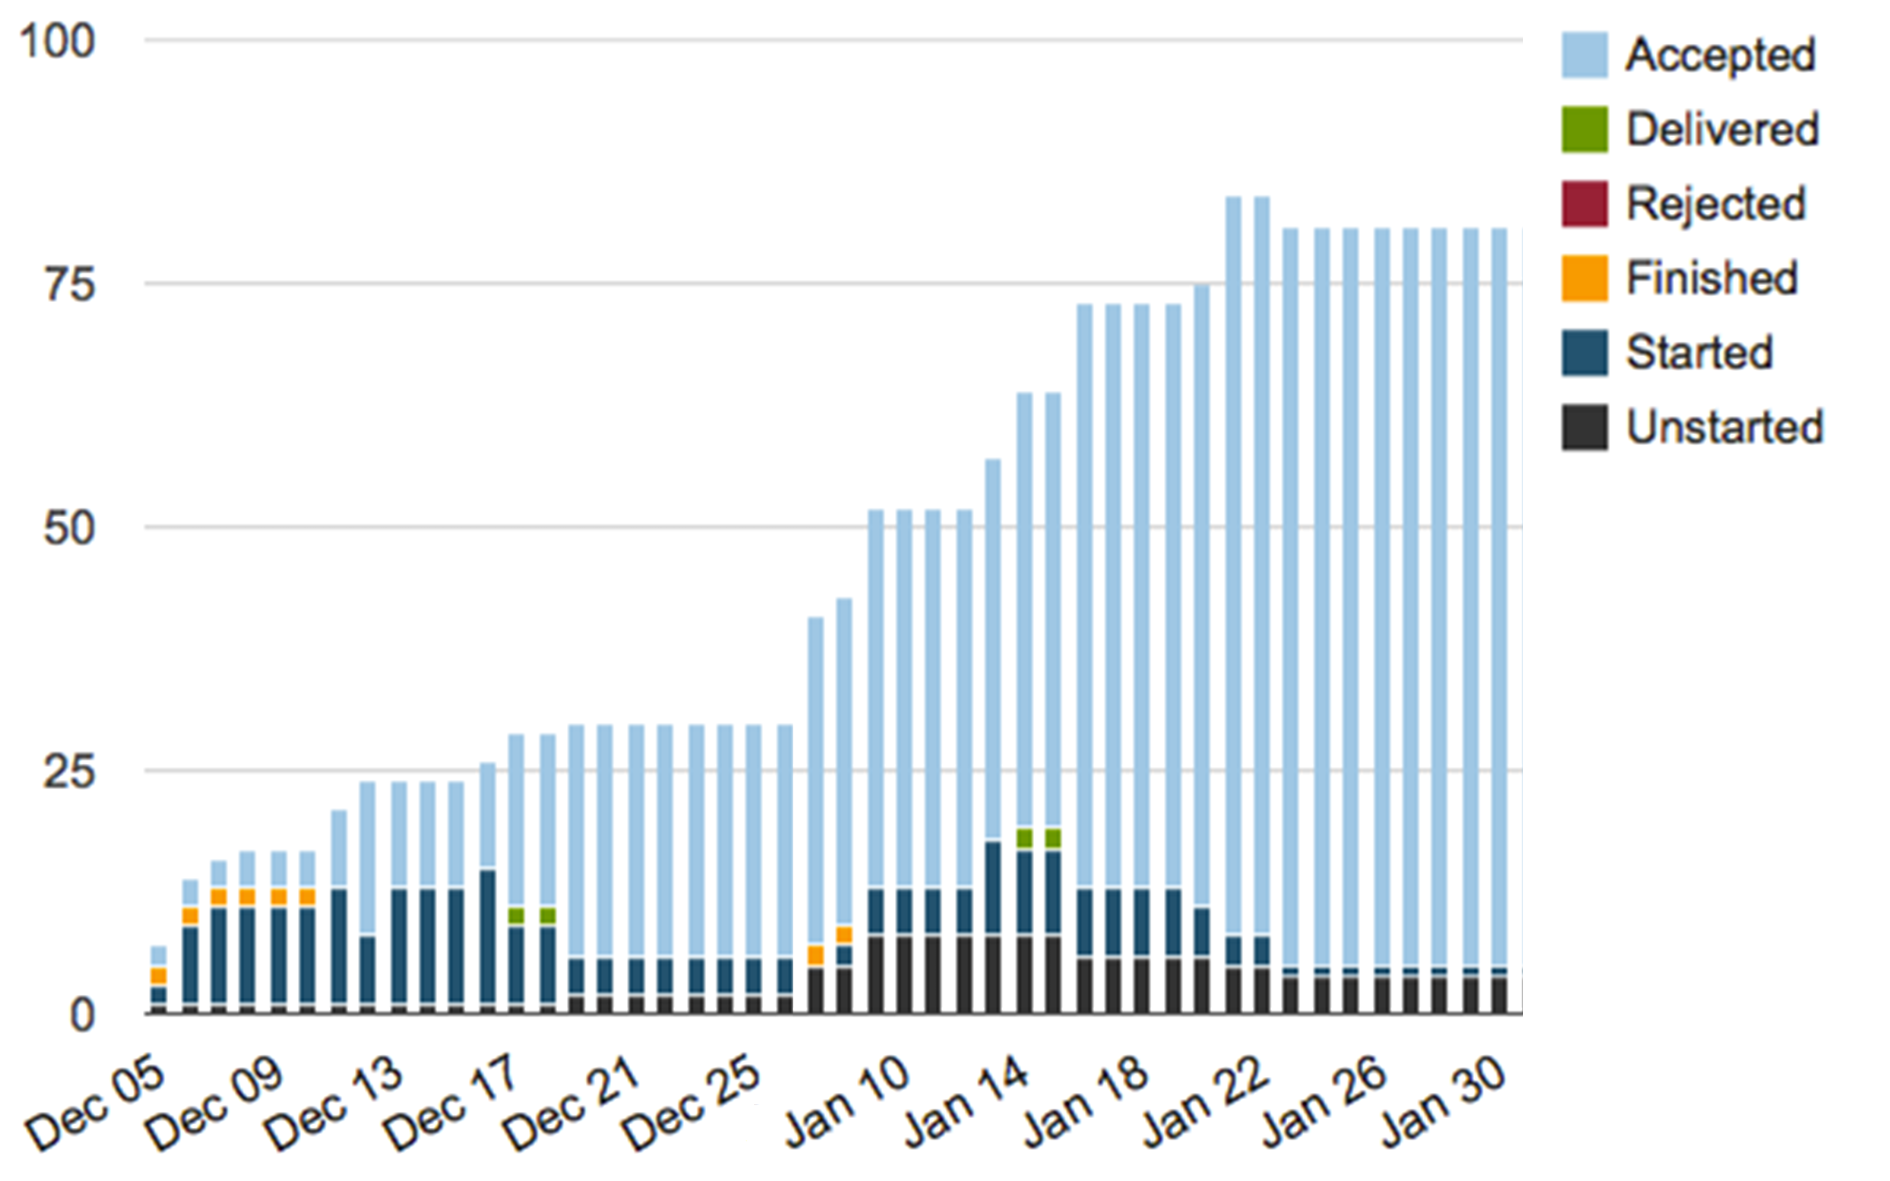
\includegraphics[width=.6\textwidth]{Pictures/burndown-compiled}
	\caption{Von PivotalTracker generiertes Burndown-Chart \label{fig:BurndownCompiled}}
\end{figure}

	Aus der Tendenz ist ersichtlich, dass die Sprint-Velocity unter Vernachlässigung der Ferienzeit stetig  bis zur Deadline zunahm.